\chapter{Qubit}
\noindent \lecture{12}{16/11/2021}
\section{Tipologie di qubit}
Nell'ambito dei qubit superconduttivi possiamo individuare tre tipologie di qubit:
\begin{itemize}
    \item \textbf{Phase qubit} (\textit{current biased Josephson junction});
    \item \textbf{Charge qubit} (\textit{single cooper pair box}: CPB);
    \item \textbf{Flux qubit}.
\end{itemize}
Queste tre tipologie si ramificano poi in varie sottocategorie di qubit: fra questi si noti il caso della tecnologia \textbf{XMON} (attualmente la più diffusa) che è un'evoluzione del \textbf{TRANSMON} che, a sua volta, deriva dal \textbf{CPB}.

\subsection{Phase qubit}
Studiamo ora il phase qubit e consideriamo una giunzione Josephson: abbiamo visto che possiamo approssimarla a un circuito con capacità e giunzione ideale:
\begin{figure}[!ht]
  \begin{center}
    \begin{circuitikz}
      \draw (0,0)
      to[C] (0,2) % The L source
      to[short] (2,2)
      to[barrier] (2,0) % The resistor
      to[short] (0,0);
    \end{circuitikz}
  \end{center}
\end{figure}
\newline
A questo punto andiamo ad aggiungere una corrente di bias $I_b$:
\begin{figure}[!ht]
  \begin{center}
    \begin{circuitikz}
      \draw (0,0)
      to[C] (0,2) % The L source
      to[short] (2,2)
      to[barrier] (2,0) % The resistor
      to[short] (0,0)
      (0.5,0) -- (0.5,-0.5) -- (-1.5, -0.5)
      to[ioosource=$I_b$] 
      (-1.5,2.5) -- (0.5,2.5) -- (0.5,2);
    \end{circuitikz}
  \end{center}
\end{figure}
\newline
Cerchiamo di capire quale sia la differenza tra il circuito LC e il circuito LC con una corrente di bias.
Abbiamo già visto che l'hamiltoniana di un oscillatore armonico LC può essere scritta come:
\begin{equation*}
     H = 4E_C  n^2 + \frac{1}{2} E_L  \delta^2 %= E_C \frac{P^2}{\hbar ^ 2 }+ \frac{1}{2}E_L \delta^2
\end{equation*}
Se sostituisco l'induttore $L$ con un induttore Josephson, devo scrivere la relazione che lega la corrente $I$ al flusso relativo alla giunzione:
\begin{equation*}
    I = I_0 \sin \delta = I_0 \sin \left( 2\pi \frac{\Phi}{\Phi_0}\right)
\end{equation*}
A questo punto siamo in grado di risolvere il circuito esplicitamente a partire dalle equazioni del moto. 
Supponiamo adesso che la corrente di bias sia nulla ($I_b=0$) e andiamo subito a calcolare l'hamiltoniana.
Sappiamo già qual è l'energia cinetica legata al circuito, dobbiamo ricavare ancora l'energia potenziale legata alla giunzione Josephson. In realtà avevamo visto anche questa, arrivando a:
\begin{equation*}
    U = \int^t_{-\infty} dt\, I(t) V = E_J ( 1 -\cos \delta) = \frac{I_0 \Phi_0}{2\pi}(1-\cos \delta)
\end{equation*}
Rimuovendo il termine $E_J$ costante dall'energia potenziale (si tratta solo di riscalare le energie per un valore costante), possiamo scrivere l'hamiltoniana come:
\begin{equation*}
     H = 4E_C  n^2 - E_J \cos  \delta
\end{equation*}
Possiamo riscrivere l'hamiltoniana in termini del momento delle coppie di cooper:
\begin{equation*}
     H = 4E_C \frac{ p^2}{\hbar^2}- E_J \cos{\delta}
\end{equation*}
Questa hamiltoniana descrive un oscillatore anarmonico:
\begin{figure}[!h]
    \centering
    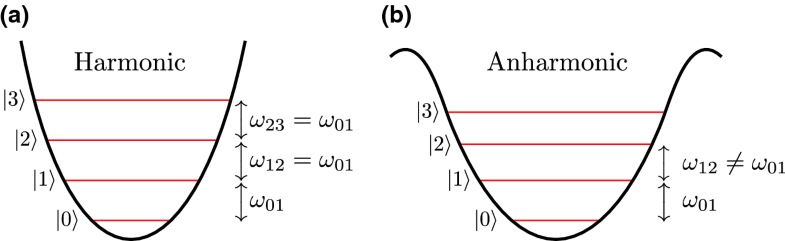
\includegraphics[width=0.7\textwidth]{images/hanarmonicity.png}
\end{figure}
\newline
In effetti, nel limite per $\delta \rightarrow 0$ possiamo mantenere solo il primo ordine dell'espansione di Taylor del secondo termine per riottenere un'hamiltoniana armonica:
\begin{equation*}
     H \approx 4 E_C \frac{ p^2}{\hbar ^ 2} + \frac{E_J \delta^2}{2}
\end{equation*}
La frequenza di oscillazione diventa (introducendo $L_{J0} = \frac{\hbar}{2eI_0}$):
\begin{equation*}
    \omega_0 = \frac{1}{\sqrt{LC}}\longrightarrow \frac{1}{\sqrt{L_{J_0}C}}
\end{equation*}
A questo punto lasciamo cadere l'assunzione per cui $I_b=0$:
\begin{equation*}
    I_b = \frac{\hbar}{2e}C\ddot \delta + I_0 \sin \delta 
\end{equation*}
Avremo i due termini energetici (li otteniamo ricavando la lagrangiana del sistema):
\begin{align*}
    K (\dot \delta) &= \left( \frac{\hbar}{2e}\right)^2 \frac{C}{2}\dot \delta ^ 2  \\
    U ( \delta, I ) &= \frac{\hbar }{2e}\int^t _{-\infty} d\delta\, (I_0 \sin \delta - I_b)  = \frac{\hbar}{2e} I_0 (1-\cos\delta ) - \frac{\hbar}{2e}I_b\delta
\end{align*}
Con una serie di passaggi poco interessanti, possiamo arrivare a riscrivere l'hamiltoniana completa del circuito:
\begin{equation*}
     H = \left(\frac{\hbar}{2e}\right)^2C{\dot\delta}^2 - E_J \cos{\delta} - I \frac{\delta\hbar}{2e}
\end{equation*}
Rimane da rendere più chiaro il primo termine.
Da adesso in poi $E_C$ è l'energia di una singola coppia di cooper ($E_C = \frac{2e^2}{C}$) il che porta a un'energia cinetica scritta come: $K=E_C \frac{p^2}{\hbar^2}$.
Dalla lagrangiana del sistema possiamo definire il momento:
\begin{equation*}
    \partialderivative{L}{\dot \delta} = \frac{\hbar^2\dot\delta}{2E_C} = p
\end{equation*}
Sapendo, per l'effetto Josephson AC, che: $V = \frac{\hbar}{2e}\dot \delta$, possiamo riscrivere:
\begin{equation*}
    \partialderivative{L}{\dot \delta} = \left(\frac{\hbar}{2e}\right)^2C \dot \delta = \frac{\hbar}{2e}CV = \frac{\hbar}{2e}Q = \hbar n
\end{equation*}
Con $n$ che rappresenta il numero di coppie di Cooper.
Con quest'ultima informazione otteniamo una nuova rappresentazione per l'hamiltoniana:
\begin{equation*}
     H = E_C  n^2 - E_J \cos{\delta} - I_b\frac{\delta\hbar}{2e}
\end{equation*}